\section{Development Activities}
\label{sec:development_activities}
\lhead{\thesection \space Development Activities}

This chapter covers three activities that the author improved their competence in over the course of the project. Each activity is detailed in the context of one architectural layer, such as \textit{Software} or \textit{User Interaction}. The level of competence at the beginning of the project is being described first, followed by the improvement during the project, as well as how the improvement came to be in the context.

\subsection{User Interaction Implementation}
\label{ssec:user_interaction_implementation}

At the beginning of the project, I possessed a skill level of Level 1 when it came to implementing processes in the context of \textit{User Interaction}. I was able able to implement static forms of elements that a user can interact with. To do so, a limited amount of interactive components could have been made use of.
\newline
As planned in the personal development plan, I wanted to make use of innovative technologies to enhance the experience of the user interacting with the developed product. It wanted to familiarise myself with simple yet productive techniques and frameworks to be used in terms of User Interaction.
\newline
The project provided an excellent base to expand my skills regarding this topic. \textit{React Native}, which is first and foremost a framework for frontend application, provided plenty of possibilities to implement components that a user would ultimately have to interact with. The implemented component which shows this acquired skill the most is the \textit{WizardProcess} component. This component is the main part of a component structure that creates a Setup Wizard. This Wizard guides a user through the steps of creating a poll, which is the main goal of the \textit{Vote4Fun} extension. The \textit{WizardProcess} component is responsible for showing the appropriate component at each stage of the Wizard, for example a text field for the user to enter the name of the poll or a date picking component for when the user has to set a due date.
\newline
This component was designed with simplicity in mind. To create a poll, a user is required to enter a large set of values as information. Having the user enter all of these values in a single view would get convoluted and overfull, decreasing user satisfaction. Instead, a user is only presented with at most three options at any time: enter a value, take a step forward or take a step back. Figure \ref{fig:wizard_due_date_screenshot} shows an example of such a limited view. The user only has the option to enter a due date or to go back a step. Even the option to move forward is disabled in this example, since the value the user entered is not valid.

\begin{figure}[H]
    \centering
    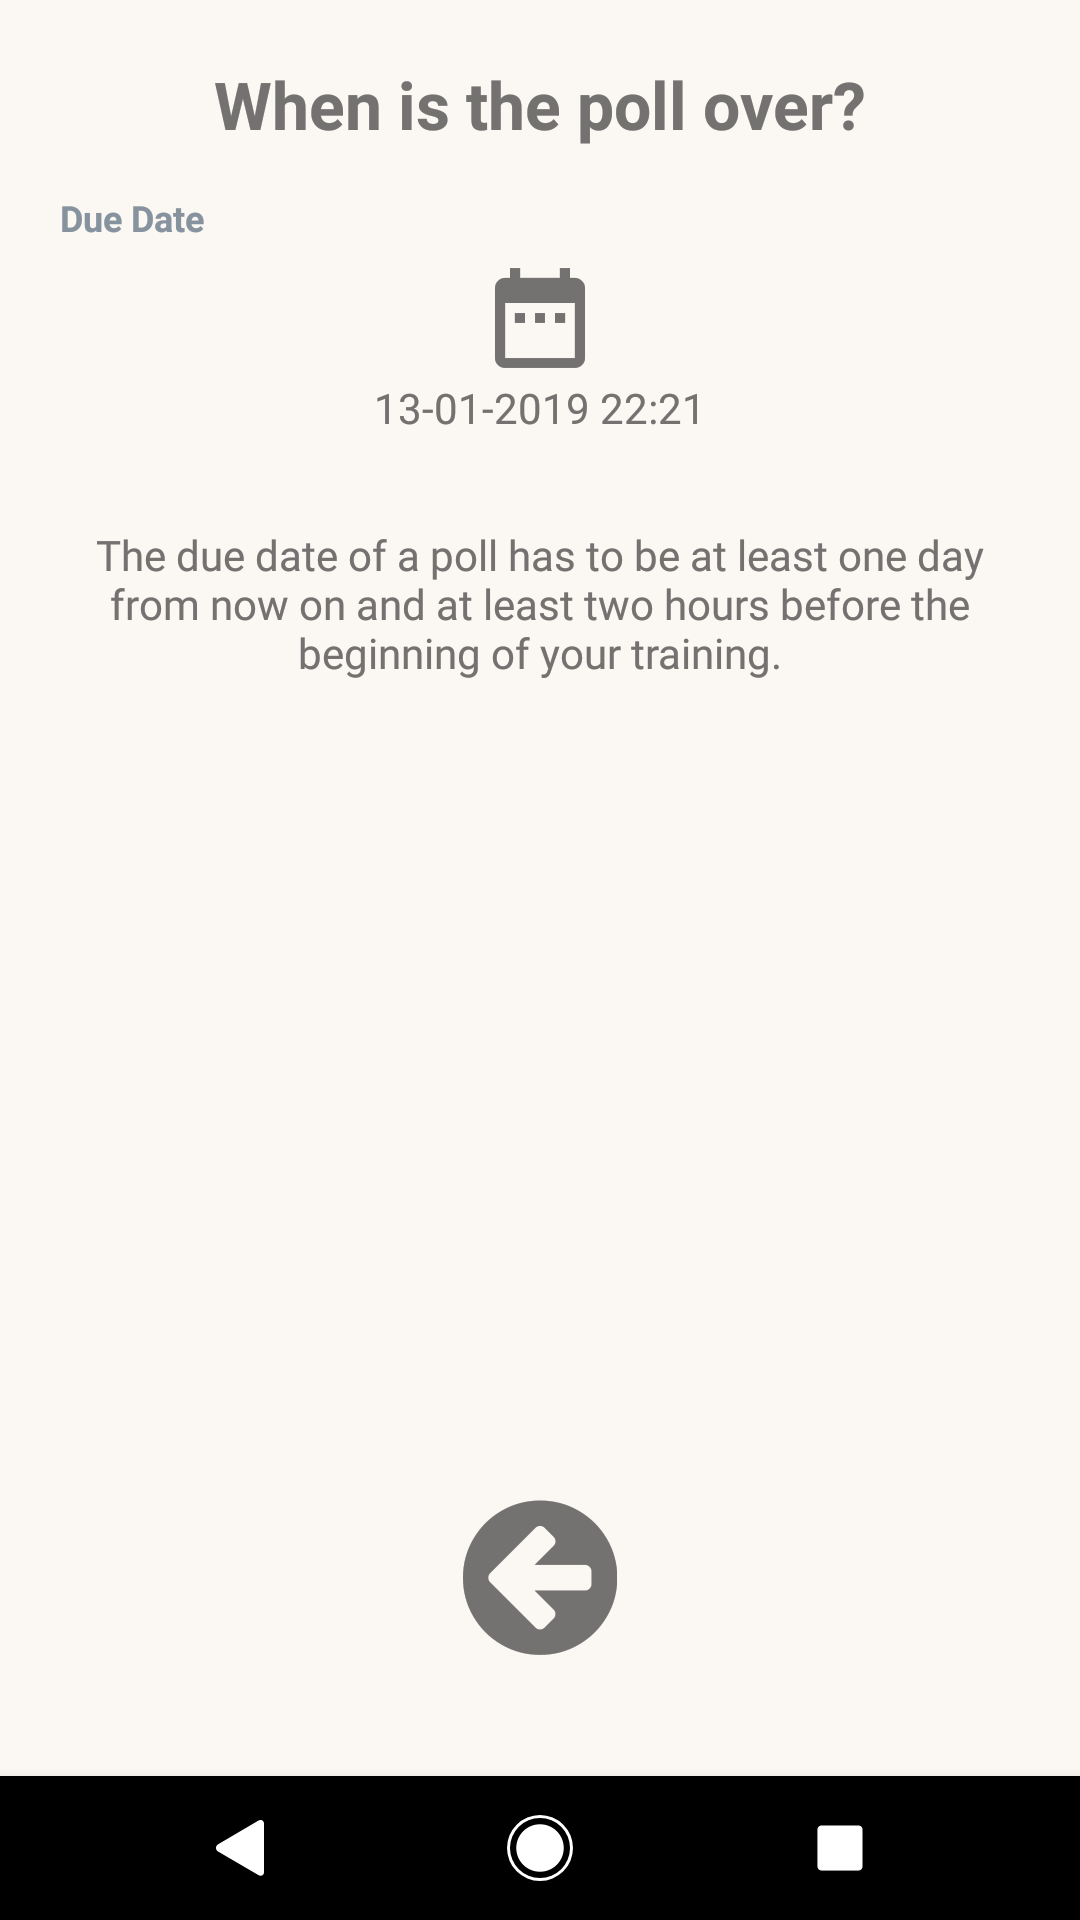
\includegraphics[width=0.5\textwidth]{images/wizard_due_date_screenshot.png}
    \caption{Setup Wizard Due Date Entry Screenshot}
    \label{fig:wizard_due_date_screenshot}
\end{figure}

The idea to make use of a Setup Wizard combined with the framework of \textit{React Native} is simple yet really efficient. The component-based nature of \textit{React Native} allows it to quickly change views presented to the user. Furthermore, each component presented is also a standalone component in development code, removing interdependency between components.
\newline
Aside from implementation of \textit{User Interaction}, I also wanted to familiarise with the possibilities of testing graphical user interfaces and \textit{User Interaction} in general. As a research I have taken a look at various frameworks which support testing graphical user interfaces of \textit{React Native} applications. This research can be found in the Appendix of the Group Dossier of this project.
\newline
Part of researching these testing frameworks was the interaction with the deployed application. Using various drivers, I was able to write tests that reference some properties of interactive components. For example, two of the frameworks made use of \textit{Accessibility Labels}, a property available in native \textit{Android} applications, while others required adding references to user interactive components. In any case, I was able to simulate user input and interactivity as part of end-to-end tests and I am now able to develop test-driven application in \textit{React Native} and other similar frameworks.

\subsection{Software Design}
\label{ssec:software_design}

Since I have worked on multiple different projects before this one, I was able to design software systems from scratch. The skill to come up with prototypes and to design both for implementation and tests of new and existing components of a system is given, as specified in Level 2 of the BOKS model.
\newline
I wanted to improve my skill by developing the ability to design complex software systems, consisting of new, existing and perhaps deprecated components. Such a software system was supposed to satisfy both stakeholders and quality assurance, including a proper test strategy.
\newline
To prove the improvement of my skills, I designed the component structure that makes up most of the \textit{Vote4Fun} extension. This structure can be seen in form of a component diagram in Figure \ref{fig:component_diagram}.

\begin{figure}[H]
    \centering
    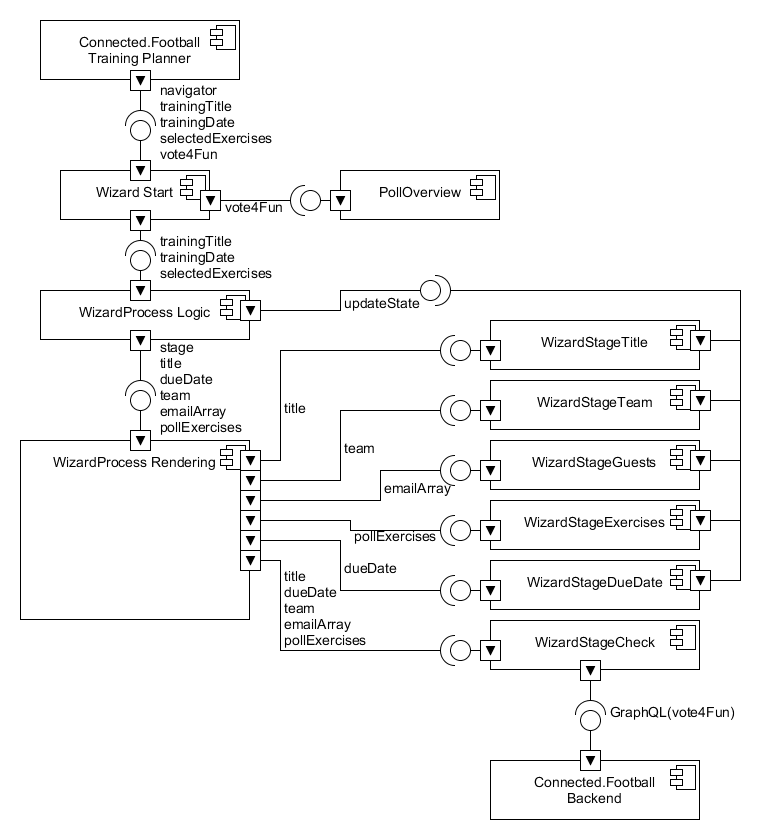
\includegraphics[width=\textwidth]{images/component_diagram.png}
    \caption{\textit{Vote4Fun} Component Diagram}
    \label{fig:component_diagram}
\end{figure}

As it can be seen, the system consists of many different components. Of these components, some were developed by the project team and some were already existing and available, such as the \textit{Connected.Football} Training Planner component. The idea behind this design was to create a complex structure of components that provide a certain result that is than returned to another system or component. In this example the existing system is the already developed \textit{Connected.Football}. The other components can act independently as a structure and can therefore be called from almost any point in the rest of the application, satisfying the need to be compatible with existing components. Since the structure is mostly independent, it is also possible to work with already existing yet deprecated components, since the structure itself only returns a result, in this case a \textit{GraphQL} mutation. How this result is handled is up to the receiving component. The newly designed components are not dependent on any business logic implemented by existing and potentially deprecated components.
\newline
The amount of components also makes it possible to conduct proper quality assurance. First of all, each component is largely independent from any other component, thanks to the component-based approach of \textit{React Native}. This way, any developed component is open to unit and component testing. Given the fact that most of the components are designed as functional components, this becomes a matter of inputting properties to see if the returned result is as it was expected.
\newline
Furthermore, the structure defines a successive process that creates a Setup Wizard. Such a Wizard and the interaction within it are a great example of a software system that should be end-to-end tested. As part of a research paper I have written during this project, the possibilities to test a \textit{React Native} application this way were considered.
\newline
Overall, I am now able to construct complex systems and to integrate said system into an already existing structure of components. I am also able to consider how interdependent these components should be while designing these aforementioned systems.

\subsection{Software Implementation}
\label{ssec:software_implementation}

Before the project, I was able to build software system, both independent and more complex systems with multiple subcomponents, including the ability to integrate the developed systems into existing software and environments. The ability to perform unit and system tests regarding the performance and integrity of the built products was also present. This is equivalent to Level 2 of the BOKS model.
\newline
I wanted to learn how to build software on an already designed architecture. The nature of the project was a perfect base for this learning goal, since a main part of the development work revolved around \textit{React Native}, a framework designed to make use of reusable components. Utilising existing components, both developed by the customer and available through open source, as well as writing and integrating new components was a good practise to reach this learning goal.
\newline
As mentioned in \textit{\ref{ssec:software_design} \nameref{ssec:software_design}}, I designed the component structure that would eventually become the Setup Wizard that is at the heart of the \textit{Vote4Fun} extension. Using this as a base for implementation, the components were implemented accordingly. During development, it was paid attention to the fact how the newly implemented components interact with the already existing system, making sure to not alter any existing sources.
\newline
One thing that was made heavily use of is the framework \textit{recompose}. This framework allowed the complete separation of business logic and rendering of the Setup Wizard, including the possibility to create callback methods for other components used by the Wizard. This way, it was possible to introduce existing components, which were managed using the \textit{Node.js} package manager, into the component structure without having to make sure that all components respond accordingly. Each introduced component was used only where appropriate, without altering the behaviour of any other component, neither of those implemented by the project team nor already existing ones.
\newline
Gaining skills in test automation was also a skill that should be advanced by participating in the project. While test automation was not implemented as extensively as it is done for example in \textit{Continuous Integration}, I researched how automatic testing can be done fast and efficiently while making use of \textit{React Native}.
\newline
As part of my research I have worked with \textit{Jest}, which takes a snapshot-based approach to automated testing. Each time a component is changed during implementation, the tests can be ran to see if the component changed in terms of rendering. If it does, a developer can decide whether this change is intentional or if something has gone wrong during development. If everything is in order, the result is stored to be used during the next test iteration. This form of test can be automated. For example, it could run in a test pipeline, running every time a change is committed to the source files of a component.
\newline
In conclusion, I am now able to implement software systems given a design as a base for implementation. Furthermore, I am able to devise and implement tests that can run automatically, responding to change.